\documentclass{bioinfo}
\copyrightyear{2016} \pubyear{2016}

\access{Advance Access Publication Date: Day Month Year}
\appnotes{Manuscript Category}

\begin{document}
\firstpage{1}

\subtitle{Data and text mining}

\title[mimic-code]{MIMIC Code Repository: tools for deriving clinical concepts}
\author[Johnson \textit{et~al}.]{Alistair E. W. Johnson\,$^{\text{\sfb 1,}*}$ and Tom Pollard\,$^{\text{\sfb 1}}$}
\address{$^{\text{\sf 1}}$Institute of Medical Engineering \& Science, Massachusetts Institute of Technology, Cambridge, 02139, USA %and \\
%$^{\text{\sf 2}}$Department, Institution, City, Post Code, Country.
}

\corresp{$^\ast$To whom correspondence should be addressed.}

\history{Received on XXXXX; revised on XXXXX; accepted on XXXXX}

\editor{Associate Editor: XXXXXXX}

\abstract{\textbf{Motivation:} Secondary analysis of electronic health records is increasingly becoming necessary to derive insights into clinical care. Retrospective studies frequently require similar clinical concepts, and an open standardized tool for deriving these concepts is desirable to ensure the consistency and efficiency of future studies.\\
\textbf{Results:} We present the MIMIC Code Repository: an open access repository with code for deriving a large number of clinical concepts in the MIMIC database. Concepts include severity of illness scores, organ failure indices, duration of treatments such as ventilation and dialysis, among others. \\
\textbf{Availability:} The actively developed code is freely available on GitHub ( ?? ) and a PhysioNet mirror with stable versions has also been made available ( ?? ).\\
\textbf{Contact:} \href{aewj@mit.edu}{aewj@mit.edu}\\
\textbf{Supplementary information:} Supplementary data are available at \textit{Bioinformatics} online.}

\maketitle

\section{Introduction}

\subsection{Knowledge gaps in intensive care}

% Here talk more about the issues in intensive care. Unproven therapies etc. Then lead on to why further research is needed. 

% Discuss creating community around the data. Creating a reproducible workflow for research.

Set out some of the problems and our knowledge gaps. Emphasise importance of research. For example, preventable mortality, reducing length of stay, preserving resources etc. Introduce some studies that have used MIMIC. Explain that code has been written independently on each occasion. 

To address these gaps in our knowledge, key steps are needed. Available data. Studies that can be reviewed and improved and repeated over new datasets. Facilitated by code sharing etc..

Lead on to say how data and code shared together a collaborative research workflow. Explain benefits of creating a repository of shared data. Supports reproducibility.  Also allows researchers to work closely with us - the database developers - while making this task manageable given the size of the community. 

To combine the efforts of the community, to promote collaborative development, stepwise improvement etc, we have created a shared repository for code. Leads on to...


\subsection{Data availability}

% Background to MIMIC. From original version to now. Talk about how code sharing has changed.

Introduce the Medical Information Mart for Intensive Care (MIMIC-III) database is a large collection of information pertaining to in-patient stays at intensive care units (ICU) in the Beth Israel Deaconess Medical Center, Boston, MA, USA \cite{mimiciii}. 

% Cite and address the points in: http://journals.plos.org/plosbiology/article?id=10.1371/journal.pbio.1001745

% This section can go into more detail about MIMIC-III. Give outline of the data. Explain how data can be used. etc.

The latest version of MIMIC-III, v1.4, houses data spanning 11 years between 2001 and 2012, and is made freely available to researchers upon signing of a data use agreement and proof of a human studies training course. 

MIMIC-III is an unmatched research resource in the area of clinical informatics that not only promotes crowdsourcing of knowledge generation but, more importantly, allows investigators to easily reproduce and expand upon results that utilise the data. 

Also introduce the work that we are doing on eICU. Say that code could be generalised.

\subsection{MIMIC Code Repository}

% Discuss what kind of code should be shared and why, leading on to reproducibility

Analysis performed on the database often requires definition of clinical concepts, including severity of illness scores, vasopressor usage, organ failure assessments, and treatments delivered. To date these concepts have been extracted independently by researchers. 

The lack of a centralized repository for code results in repetition of work, inconsistency, and increases the probability of errors in the extraction process. 

The MIMIC Code Repository aims to standardize the definition of key clinical concepts and facilitate future studies on the MIMIC-III database. The package also provides code for importing the MIMIC-III database locally in a variety of software packages.

\begin{methods}
\section{Methods}

\subsection{The need for collaboration}

% Explain importance of the code. Why is it necessary. Who will use it?

% Discuss how multidiscplinary team needed to build the data and code. Frequent trips to the hospital etc.

Basically explain why our approach is important. Need to work together to identify  and address issues. Explain how public issue tracker allows research related questions to be raised. For example, community demand to develop severity of illness scores. Already seen multiple requests to merge code.

Interesting - provides a mechanism for researchers to work together, while still retaining a level of control over projects because code is developed in isolated chunks.

Could also mention how Stackoverflow is being used for discussion. Has this happened for other research projects? I guess so, but would be interesting to check.

Could reference the NEJM research parasite controversial paper, and say that while language not well chosen, feel that encouraging community to work with database developers has benefits.

\subsection{Identifying and addressing issues}

% The introduce the following subsections. i.e. what are the core chunks of code in the repo?
The MIMIC Code Repository utilizes structured query language (SQL) to define the concepts as MIMIC-III  is a relative database. The code is written primarily using PostgreSQL 9.5.0, and has been tested to be compliant with Oracle.

% Need to emphasise how much work has gone into creating the code

% One of challenges of developing code is understanding the underlying data. Involves regular discussion with the clinical teams.

% Need to emphasise that the code will be reused widely in research studies.

A prerequisite for using the SQL code in the \emph{mimic-code} package is access to MIMIC-III in a database management system (DBMS). The repository provides access to scripts which facilitate building the database in PostgreSQL, MySQL, and Oracle. These scripts create the tables, load the data, and provide indices for improved performance. A tutorial for creating a local PostgreSQL instance of MIMIC-III is also available in the repository.

Aside from importing MIMIC-III into a DBMS, the \emph{mimic-code} package facilitates:

\begin{itemize}
\item inferring treatment using surrogate information
\item deriving severity scores
\item deriving organ failure scores
\end{itemize}

\subsection{Focusing efforts}

Introduce the following subsections, explaining some sample areas that are being addressed by the code. For example, identifying vasopressor use, assessing severity of illness, etc. Then briefly introduce some other areas that are under development. 

\subsubsection{Introducing new researchers}

New datasets can be intimidating and take time to learn. Seek to provide introduction to the data. Could also highlight how cookbook code is being used in tutorials to introduce new users to the database in a friendly way.

\subsubsection{Interpreting treatment}

% more detail about specific issue being addressed by the code. more detail about performance of the code.

Studying the impact of treatment on patient health or adjusting for the use of treatment during a patient's care is a common task in secondary analysis of electronic health records. The \emph{mimic-code} package provides start and stop times for mechanical ventilation, dialysis, and various vasopressors. An example of these durations is provided in Figure \ref{fig:treatment}.

% could also mention here that code is provided for views that ease interpretation of data.

\subsubsection{Severity of illness}

% more detail about specific issue being addressed by the code. more detail about performance of the code.

% what are the challenges of creating the scores?

Quantifying the severity of illness for a patient is an integral part of retrospective analysis as it allows for investigation of concepts of interest in comparable patient populations. 

There are five severity of illness scores currently implemented in the \emph{mimic-code} package: APS-III \cite{aps}, SAPS \cite{saps}, SAPS-II \cite{sapsii}, SOFA \cite{sofa} and OASIS \ref{oasis}. The performance of these scores in discriminating hospital mortality is shown in Figure \ref{fig:SevScoresOverTime}. More detailed comparison of the severity scores is provided in the supplementary material.

\begin{figure}[!tpb]%figure1
\centerline{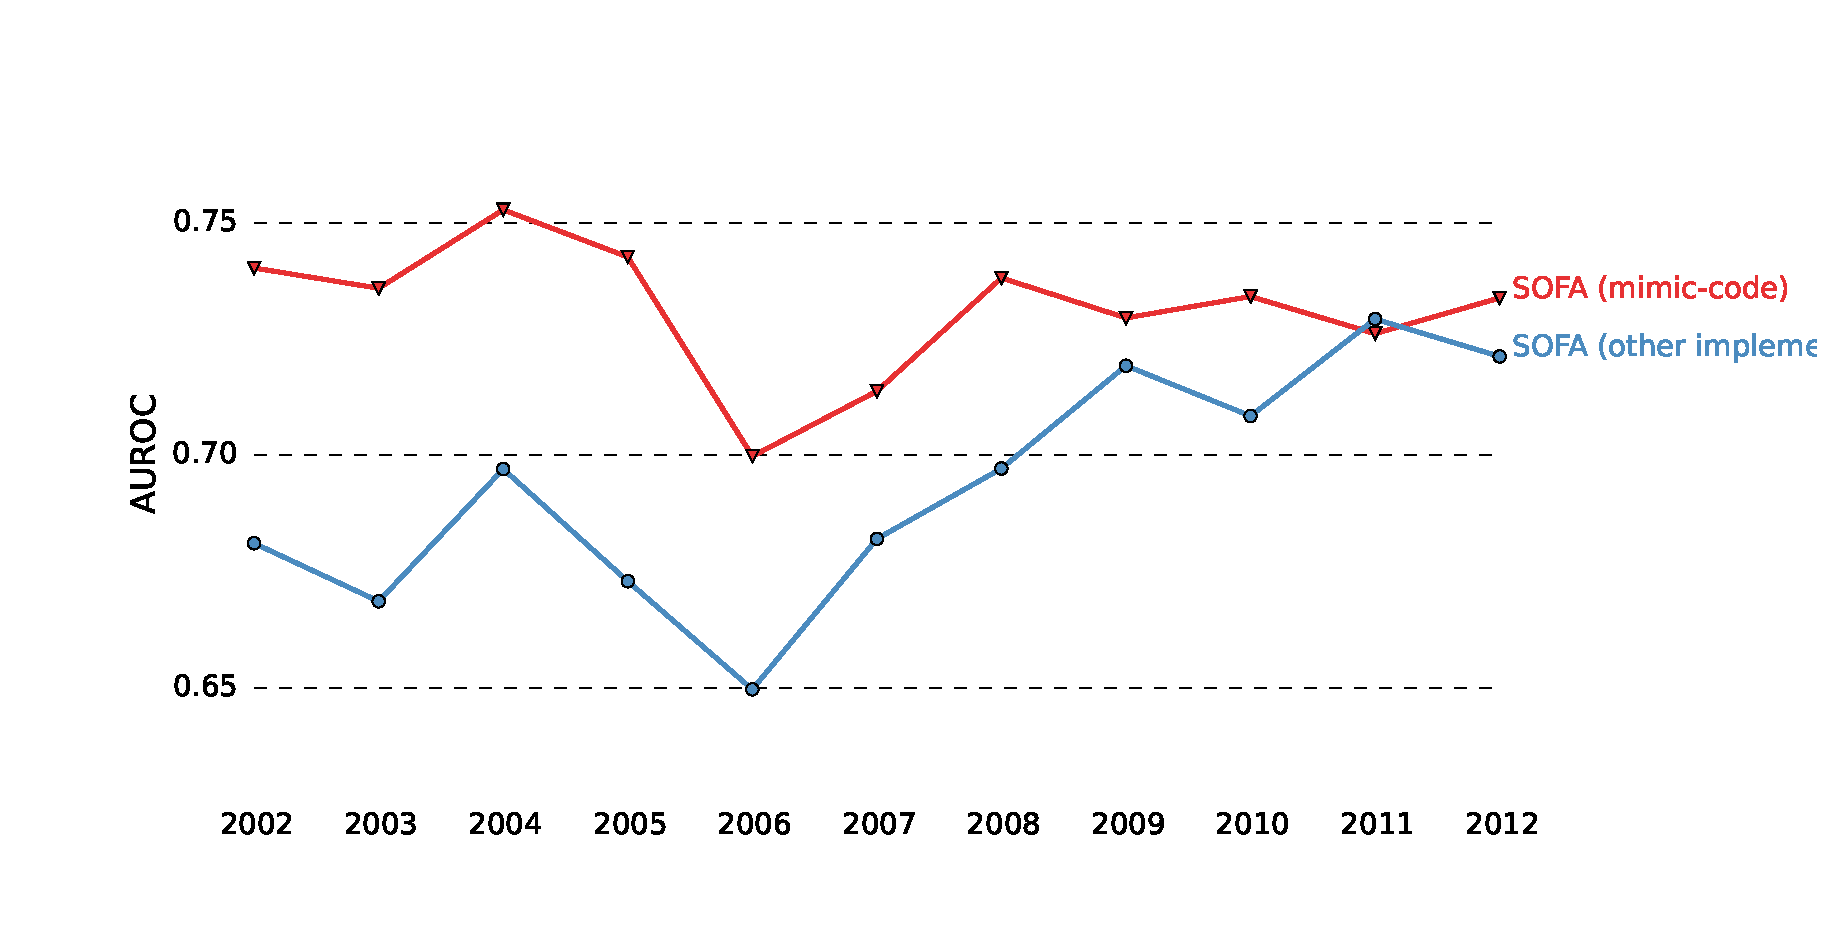
\includegraphics[width=0.5\textwidth]{SOFA.eps}}
\caption{Discrimination of two implementations of SOFA across fiscal years as measured by the area under the receiver operator characteristic curve (AUROC).}\label{fig:SevScoresOverTime}
\end{figure}

In addition, scores used to measure the failure of a specific organ are also available for the hepatic (MELD \cite{meld}) and renal (KDIGO \cite{kdigo}, RIFLE \cite{rifle}) systems.

%\begin{table}[!t]
%\processtable{This is table caption\label{Tab:01}} {\begin{tabular}{@{}llll@{}}\toprule head1 &
%head2 & head3 & head4\\\midrule
%row1 & row1 & row1 & row1\\
%row2 & row2 & row2 & row2\\
%row3 & row3 & row3 & row3\\
%row4 & row4 & row4 & row4\\\botrule
%\end{tabular}}{This is a footnote}
%\end{table}

\subsection{Code quality and sustainability}

Unit testing. To promote code quality etc, unit tests are triggered when code updates are integrated into the database. Facilitates detection of bad code, etc.

Also sustainable approach, because code is shared and maintained with the community. Means researchers leaving etc becomes less of an issue.

Link to open data supports reproducbility. Often use Jupyter Notebook to create database connection to carry out studies.

Discuss versioning? Enables older studies to be reproduced...

\subsection{Community building}

Mention datathons and cite the forthcoming paper.  Continuous review. Services like Github provide incentives for researchers to contribute.

\end{methods}

%\begin{figure}[!tpb]%figure2
%%\centerline{\includegraphics{fig02.eps}}
%\caption{Caption, caption.}\label{fig:02}
%\end{figure}

\section{Discussion}

Openly available code is a key step in improving the quality of research as it provides validity to analyses performed. There are many decisions which must be made in the data extraction process which can have a large impact on the resultant data. 

For example, when extracting the Glasgow Coma Scale (GCS), severity of illness scores assign a value of 15 when a patient is sedated, but the clinical staff record values of 3. This results in a systematic bias for sedated patients unless appropriate measures are taken to correct the recorded values. However, explanation of these steps would likely be omitted from publications. 

The MIMIC Code Repository serves as a central hub for development of clinical concepts, and the use of code contained here-in has the potential to standardize future analyses.

Discuss MIMIC datathons. Allow data to be developed at the events and reused easily. Discuss the concept of continuous peer review...code is available for everyone to see and improve. Code should be fixed before it reaches stage of publication.

Perhaps also cite: http://www.nature.com/news/2010/101013/full/467775a.html

Discuss benefits of creating a community.

Discuss collaboration and reproducibility.

Highlight benefits of having an issue tracker. Allows research code to be managed over time. 

Promotes sustainable code, which is a known issue in research. Often PhD or Postdoc writes code, then leaves, and then code is not maintained.

Discuss opportunities. Unique codebase. 

\section{Conclusion}

The MIMIC Code Repository contains code which derives a variety of useful clinical concepts which simplify analyses performed on the MIMIC database. The package is openly available and will continue to incorporate new concepts as they are calculated, allowing for rapid prototyping of clinical questions in a large retrospective database. The code is written with a modular design, and could be adapted for use with other ICU databases in a straightforward manner.  \\

\section*{Acknowledgements}

The authors would like to acknowledge Professor Roger G. Mark, the MIT Laboratory for Computational Physiology, Philips Healthcare and the Beth Israel Deaconess Medical Center for the creation of the MIMIC-III database.%\vspace*{-12pt}

\section*{Funding}

This work has been supported by grants NIH-R01-EB017205, NIH-R01-EB001659, and NIH-R01-GW104987 from the National Institutes of Health.%\vspace*{-12pt}

%\bibliographystyle{natbib}
%\bibliographystyle{achemnat}
%\bibliographystyle{plainnat}
%\bibliographystyle{abbrv}
%\bibliographystyle{bioinformatics}
%
%\bibliographystyle{plain}
%
%\bibliography{Document}


\begin{thebibliography}{}

\bibitem[Le~Gall {\it et~al}., 1984]{saps}
J.~R. Le~Gall, P.~Loirat, A.~Alperovitch, P.~Glaser, C.~Granthil, D.~Mathieu,
  P.~Mercier, R.~Thomas, and D.~Villers (1984) ``A simplified acute physiology score
  for {ICU} patients,'' {\it Critical Care Medicine}, {\bf ~12}, ~975--977.

\bibitem[Le~Gall {\it et~al}., 1993]{sapsii}
J.~R. Le~Gall, S.~Lemeshow, and F.~Saulnier (1993) ``A new simplified acute physiology
  score ({SAPS-II}) based on a european north-american multicenter study,''
  {\em JAMA}, {\bf ~270}, ~2957--2963.
 
\bibitem[Knaus {\it et~al}., 1991]{aps}
W.~A. Knaus, D.~P. Wagner, E.~A. Draper, J.~E. Zimmerman, M.~Bergner, C.~A.
  Bastos, P G snd~Sirio, D.~J. Murphy, T.~Lotring, A.~Damiano, and F.~E.
  Harrell~Jr. (1991) ``The {APACHE III} iii prognostic system: Risk prediction of
  hospital mortality for critically ill hospitalized adults,'' {\em Chest},
  {\bf ~100}, 1619--1636.
 
\bibitem[Johnson {\it et~al}., 2013]{oasis}
A.~E.~W. Johnson, A.~A. Kramer, and G.~D. Clifford (2013) ``A new severity of illness
  scale using a subset of acute physiology and chronic health evaluation data
  elements shows comparable predictive accuracy,'' {\em Critical Care
  Medicine}, {\bf ~41}, 1711--1718.
  
\bibitem[Vincent {\it et~al}., 1996]{sofa}
J.-L. Vincent, R.~Moreno, J.~Takala, S.~Willats, A.~{De Mendoca}, H.~Bruining,
  C.~K. Reinhart, P.~M. Suter, and L.~G. Thijs (1996) ``{The SOFA (Sepsis-related
  Organ Failure Assessment) score to describe organ dysfunction/failure},''
  {\em Intensive Care Medicine}, {\bf ~22}, ~707--710.

%TODO:
% mimic database, MELD, KDIGO


% ARTICLE
%\bibitem[Bag {\it et~al}., 2001]{Bag01}
%Bag,M., Name2, Name3 (2001) Article title, {\it Journal Name}, {\bf 99}, 33-54.

% ARTICLE
%\bibitem[Yoo \textit{et~al}., 2003]{Yoo03}
%Yoo,M.S. \textit{et~al}. (2003) Oxidative stress regulated genes in nigral dopaminergic neurnol cell: correlation with the known pathology in Parkinson's disease. 
%\textit{Brain Res. Mol. Brain Res.}, \textbf{110}(Suppl. 1), 76--84.

% BOOK CHAPTER
%\bibitem[Lehmann, 1986]{Leh86}
%Lehmann,E.L. (1986) Chapter title. \textit{Book Title}. Vol.~1, 2nd edn. Springer-Verlag, New York.

% MAYBE AN ARTICLE
%\bibitem[Crenshaw and Jones, 2003]{Cre03}
%Crenshaw, B.,III, and Jones, W.B.,Jr (2003) The future of clinical cancer management: one tumor, one chip. 
%\textit{Bioinformatics}, doi:10.1093/bioinformatics/btn000.

% BOOK CHAPTER
%\bibitem[Auhtor \textit{et~al}. (2000)]{Aut00}
%Auhtor,A.B. \textit{et~al}. (2000) Chapter title. In Smith, A.C. (ed.), \textit{Book Title}, 2nd edn. Publisher, Location, Vol. 1, pp. ???--???.

% THESIS:
%\bibitem[Bardet, 1920]{Bar20}
%Bardet, G. (1920) Sur un syndrome d'obesite infantile avec polydactylie et retinite pigmentaire (contribution a l'etude des formes cliniques de l'obesite hypophysaire). PhD Thesis, name of institution, Paris, France.

\end{thebibliography}
\end{document}
